\section{Protocolo}

\subsection{KDF chains}\label{sec:KDF}
KDF Chains faz parte do \emph{core} de um dos principais métodos, \emph{Double Ratchet} (secção \ref{sec:DoubleRatchet}), necessários para manter o \textbf{Signal} seguro.
Este algoritmo recebe um \textbf{segredo} e uma \textbf{chave aleatória KDF} e dados de \emph{input} e retorna um \emph{output} indistinguível de um \emph{random}, isto se a chave não for conhecida.
O termo \emph{KDF Chain} é usado quando parte do \emph{output} de uma \emph{KDF} é usado para substituir a \textbf{chave aleatória KDF}, podendo assim esta ser usada para outro \emph{input}. O diagrama \ref{diagram:kdfChain} representa o processo de 3 \emph{inputs} produzindo 3 novas \emph{output keys}.


\begin{figure}[H]
\begin{center}
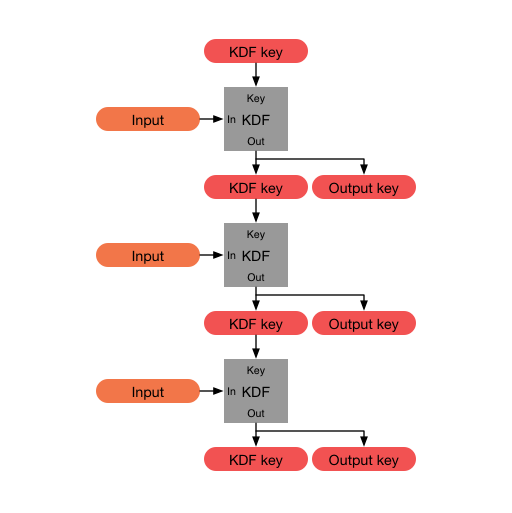
\includegraphics[width=12cm]{img/kdfChain.png}
\caption{KDF Chain com 3 inputs}
\label{diagram:kdfChain}
\centering
\end{center}
\end{figure}

Uma \emph{KDF Chain} apresenta as seguintes propriedades:

\begin{itemize}
    \item \textbf{Resiliência:} Se não houver conhecimento da chave KDF, as chaves de output aparentam ser \emph{random}. Isto mantem-se verdadeiro mesmo que o atacante controle parte dos \emph{inputs}
    \item \textbf{Forward Security:} Chaves de \textit{output} do passado aparentam ser \emph{random} para um atacante que conheceu uma chave KDF num momento futuro.
    \item \textbf{Break-in recovery:} Se os inputs futuros adicionarem entropia suficiente , as chaves \textit{output} do futuro aparentam ser \emph{random} para um atacante que conheceu uma chave KDF num momento qualquer
\end{itemize}

Numa sessão que utilize \textbf{Double Ratchet} (secção \ref{sec:DoubleRatchet}), imaginemos entre a Alice e o Bob, cada utilizador guarda 3 chaves uma para cada KDF chain: \textbf{root chain}, \textbf{sending chain},\textbf{receiving chain}. A chave sending da Alice é equivalente à chave receiving do Bob.

Por cada mensagem enviada e/ou recebida a \emph{chain} "avança" e as suas chaves de \emph{output} São usadas para encriptar e desencriptar as mensagens a este processo dá-se o nome de \textbf{symmetric-key ratchet}.

\subsection{Symmetric-key ratchet}\label{sec:symkey}
Todas e qualquer mensagem enviada ou recebida é encriptada usando uma \textbf{chave de mensagem única}. Esta chave única corresponde a uma chave de \textit{output} das \textit{KDF Chains} (secção \ref{sec:KDF} correspondentes. Chamemos a estas chaves \textit{chain keys}.

Os \textit{inputs} na KDF Chain para envio e recepção são constantes, por esta razão não fornecem \textit{break-in recovery}. As suas chains apenas garantem que cada mensagem é encriptada com uma chave única que pode ser eliminada após encriptação ou desencriptação.Calcular a próxima chave da \textit{chain} e de mensagem corresponde a um simples \textit{ratchet step} no algoritmo \textit{symmetric-key ratchet}.
O diagrama em baixo (diagrama \ref{diagram:skRatchet} demonstra a execução deste algoritmo efectuando 2 \textit{ratchet steps}.

\begin{figure}[H]
\begin{center}
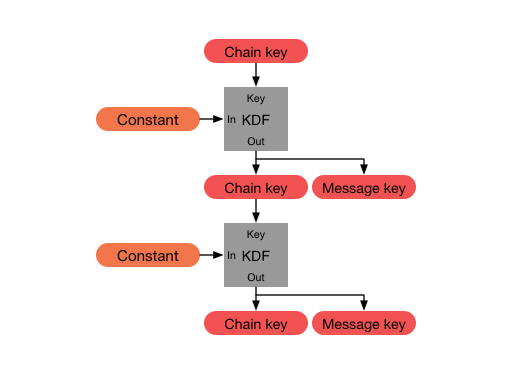
\includegraphics[width=12cm]{img/skRatchet.png}
\caption{Symmetric-key ratchet with 2 steps}
\label{diagram:skRatchet}
\centering
\end{center}
\end{figure}

\subsection{Diffie-Hellman ratchet}\label{sec:dhratchet}
Até este momento mencionamos \textit{KDF chains e Symmetric-key ratchet} ,sendo estes algoritmos necessários para o funcionamento do \textit{Double Ratchet}, no entanto estes por si só não garantem que um atacante possuindo \textit{receiving chain keys} ou \textit{sending chain keys} não consiga gerar as futuras chaves e desencriptar todas as mensagens futuras. Para evitar isto o \textbf{Signal} combina \textit{symmetric-key ratchet} com \textit{DH Ratchet}.

Para implementar um Diffie-Hellman ratchet, cada usuário gera um par de chaves Diffie-Hellman (\textit{\textbf{ratchet key pair}}). Todas as mensagens trocadas entre estes 2 usuários vão ter no header a \textbf{chave publica}. Quando o receptor recebe a chave publica do emissor é efectuado um \textbf{DH ratchet step} que consiste em substituir o actual \textbf{\textit{ratchet key pair}} por um novo par.

Este processo leva a que ambos usuários estejam constantemente a trocar as \textbf{\textit{ratchet key pair}}, desta forma se um dos usuários for comprometido, isto é, se um atacante obter a chave privada da \textit{ratchet} apenas fica comprometida uma mensagem e todas as mensagens anteriores e posteriores continuam seguras.

Os diagramas que se seguem,juntamente com o texto que os acompanham, demonstram mais especificamente o processo do \textbf{DH Ratchet}.


A Alice é 'inicializada' com a \textit{ratchet key} publica do Bob. Desta forma a chave publica da Alice ainda não é conhecida pelo Bob. A Alice executa um calculo \textit{Diffie-Helman} entre a sua \textit{ratchet key} private e a \textit{ratchet key} publica do Bob.

\begin{figure}[H]
\begin{center}
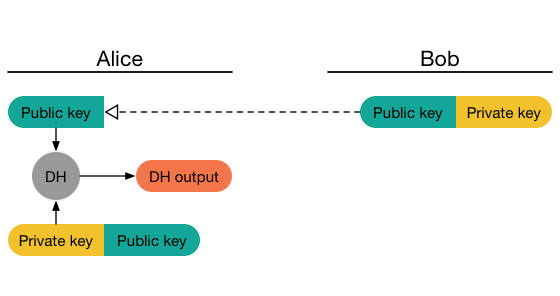
\includegraphics[width=12cm]{img/DH1.png}
\caption{}
\label{diagram:DH1}
\centering
\end{center}
\end{figure}

A primeira mensagem enviada pela Alice anuncia a sua \textit{ratchet key} publica. Quando o Bob recebe uma destas mensagens ele calcula um \textit{DH output} entre a \textit{ratchet key} publica da Alice e a sua \textit{ratchet key} privada, o que garante (através das propriedades do \textit{DH}), caso não tenha havido um \textit{middle-man} ,que seja igual ao \textit{output} inicial da Alice. O Bob ,posteriormente, substitui o seu par de \textit{ratchet keys} e calcula um novo \textit{DH output}.

\begin{figure}[H]
\begin{center}
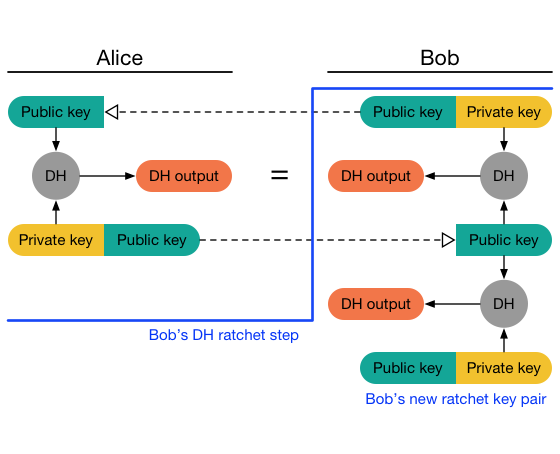
\includegraphics[width=12cm]{img/DH2.png}
\caption{}
\label{diagram:DH2}
\centering
\end{center}
\end{figure}

Uma nova mensagem vinda do Bob anuncia a sua nova \textit{ratchet key} publica. Quando a Alice receber esta mensagem vai executar um passo de \textit{DH ratchet}, substituindo a o seu par de \textit{ratchet keys} e derivando 2 novos \textit{DH outputs}, um que será equivalente ao ultimo \textit{DH output} do Bob e um novo para ser usado na próxima mensagem.

\begin{figure}[H]
\begin{center}
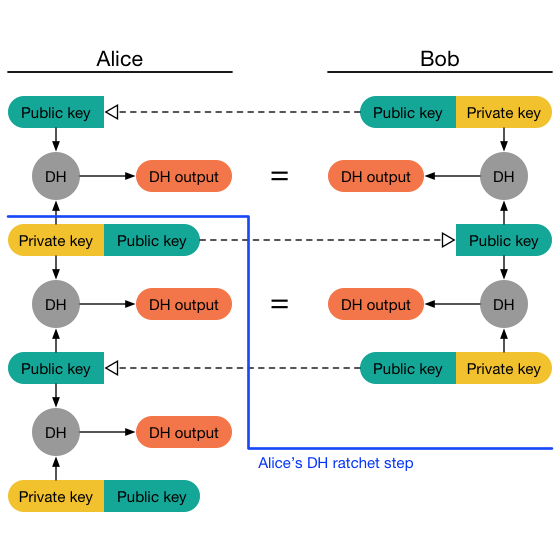
\includegraphics[width=12cm]{img/DH3.png}
\caption{}
\label{diagram:DH3}
\centering
\end{center}
\end{figure}

Uma mensagem nova por parte da Alice anuncia a sua nova chave publica. Eventualmente o Bob ira receber uma destas mensagens e executar um passo de \textit{DH ratchet} e assim sucessivamente.

\begin{figure}[H]
\begin{center}
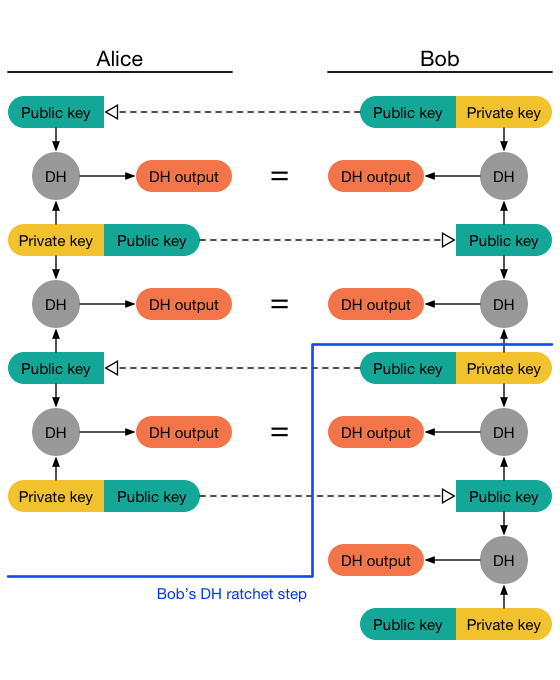
\includegraphics[width=12cm]{img/DH4.png}
\label{diagram:DH4}
\caption{}
\centering
\end{center}
\end{figure}

Os \textit{DH output} que são gerados em cada passo de \textit{DH ratchet} São usados para derivar novas chaves de envio e recepção. A imagem em baixo revisita o primeiro passo do \textit{DH ratchet} efectuado pelo Bob. Nesta imagem o Bob usa o seu primeiro \textit{DH output} para derivar a sua chave de recepção que será equivalente a chave de envio por parte da Alice.

\begin{figure}[H]
\begin{center}
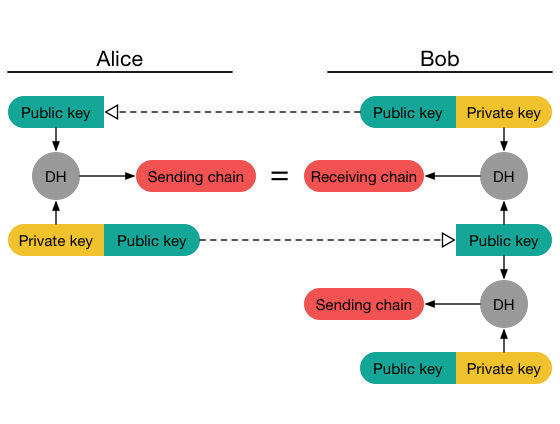
\includegraphics[width=12cm]{img/DH5.png}
\caption{}
\label{diagram:DH5}
\centering
\end{center}
\end{figure}

Sendo que os usuários efectuam \textit{"turnos"} a executar um passo do \textit{DH Ratchet} , cada um toma turnos a introduzir novas cadeias de envio:

\begin{figure}[H]
\begin{center}
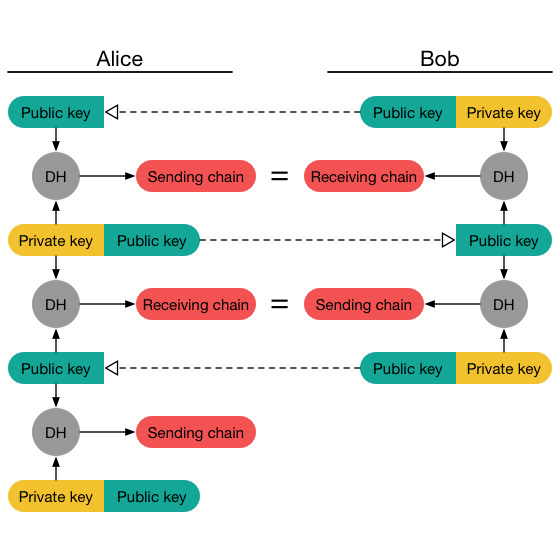
\includegraphics[width=12cm]{img/DH6.png}
\caption{}
\label{diagram:DH6}
\centering
\end{center}
\end{figure}

No entanto a imagem em cima (fig. \ref{diagram:DH6}), é uma simplificado. Em vez de se usar directamente os \textit{DH outputs}, estes são usados como \textit{KDF (\ref{sec:KDF}) inputs} para uma \textit{root chain}, sendo os \textit{KDF ouputs} da \textit{root chain} usados como chaves de envio e recepção. Usar \textit{KDF} aumenta a resiliência e \textit{break-in recovery}.

Desta forma ,um passo completo de uma \textit{DH Ratchet} consiste em atualizar a \textit{root KDF chain} $2\times$ e usar as \textit{DH output keys} como as novas chaves de envio e recepção.

\begin{figure}[H]
\begin{center}
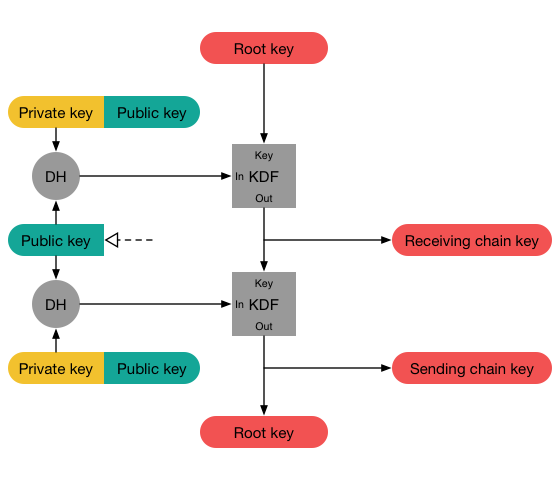
\includegraphics[width=12cm]{img/DH7.png}
\caption{}
\label{diagram:DH7}
\centering
\end{center}
\end{figure}

\subsection{Double Ratchet}\label{sec:DoubleRatchet}
\subsubsection{Para que serve Double Ratchet?}
O algoritmo \emph{Double Ratchet} é um algoritmo usado por dois usuários (aplicação móvel) na troca de mensagens encriptadas baseadas numa chave secreta partilhada entre ambos. Ambos usuários derivam uma nova chave por cada mensagem de forma a que chaves anteriores não possam ser calculadas através da chaves mais recentes. Os usuários enviam valores públicos de \emph{Diffie-Helman} juntamente com as suas mensagens. Os resultados dos cálculos de \emph{Diffie-Helman} São misturados com a chave derivada anteriormente de modo a que chaves anteriores não possam calcular chaves mais recentes. Estas propriedades garantem protecção perante das mensagens encriptadas caso exista o comprometimento das chaves de um dos usuários.

\subsubsection{Como funciona a Double Ratchet?}
A algoritmo de \textit{\textbf{Double Ratchet}} é a combinação de \textit{Symmetric-Key (sec.\ref{sec:symkey})} com \textit{DH Ratchets (sec. \ref{sec:dhratchet})} :

\begin{itemize}
    \item Quando uma mensagem é enviada ou recebida, uma passo de \textit{Symmetric-Key ratchet} é aplicado nas cadeias de envio ou recepção para derivar a nossa chave da mensagem.
    \item Quando uma nova chave \textit{ratchet public} é recebida, um passo de \textit{DH ratchet} é efetuado antes da \textit{symmetric-key ratchet} para substituir as chaves da cadeia ( \textit{chain keys})
\end{itemize}

No diagrama em baixo,\ref{diagrama:DR1}, a Alice inicializou o processo com a chave \textit{ratchet public} e um segredo partilhado (equivalente à chave raiz inicial). Na inicialização a Alice gera um novo par de chaves \textit{ratchet} e envia o \textit{DH output} para a raiz do \textit{KDF} de forma a que sejam calculadas uma nova chave raiz e uma nova chave de envio.

\begin{figure}[H]
\begin{center}
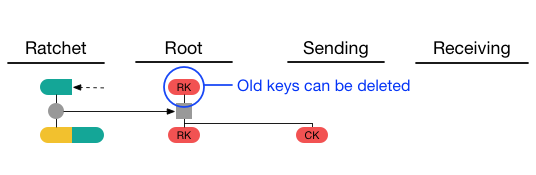
\includegraphics[width=12cm]{img/DR1.png}
\caption{}
\label{diagram:DR1}
\centering
\end{center}
\end{figure}

Quando a Alice envia a sua primeira mensagem, ela aplica um passo \textit{symmetric-key ratchet} à sua cadeia de chaves de envio, resultando numa nova chave para mensagens ( cada chave deste género possuirá um \textit{label} perante a mensagem que estas encriptam desencriptam). A nova chave da cadeia é guardada enquanto a chave para mensagem e a antiga chave de cadeia podem ser eliminadas.

\begin{figure}[H]
\begin{center}
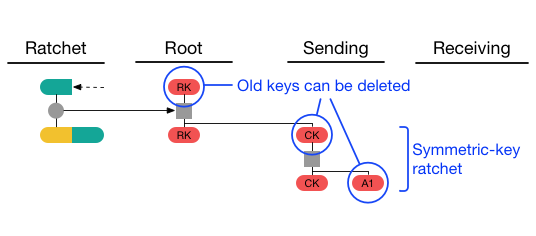
\includegraphics[width=12cm]{img/DR2.png}
\caption{}
\label{diagram:DR2} 
\centering
\end{center}
\end{figure}

Se posteriormente a Alice receber uma mensagem vinda do Bob, esta irá conter uma nova chave \textit{rachet public}. A Alice aplica um passo de \textit{DH ratchet} de forma a derivar novas chaves de envio e recepção. Posteriormente aplica um passo \textit{symmetric-key ratchet} na cadeia de recepção para obter a chave de recepção para a mensagem vinda do Bob.

\begin{figure}[H]
\begin{center}
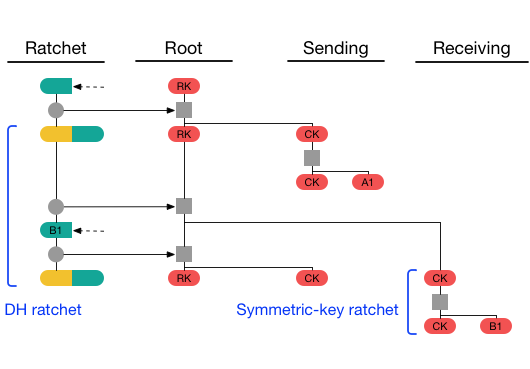
\includegraphics[width=12cm]{img/DR3.png}
\caption{}
\label{diagram:DR3} 
\centering
\end{center}
\end{figure}

Suponhamos que a Alice envia uma mensagem A2, recebe uma mensagem B2 ( com a chave \textit{rachet public} antiga ), depois envia a mensagem A3 e A4. A cadeia de envio da Alice faz 3 passos enquanto a sua cadeia de recepção apenas andou 1 passo.

\begin{figure}[H]
\begin{center}
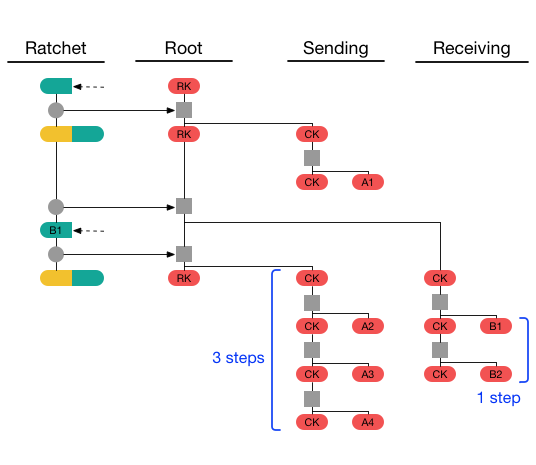
\includegraphics[width=12cm]{img/DR4.png}
\caption{}
\label{diagram:DR4} 
\centering
\end{center}
\end{figure}

Se ,posteriormente, receber a mensagem B3 e B4 com a próxima chave \textit{rachet} do Bob e em seguida enviar a mensagem A5 o seu estado final será como identificado no diagrama \ref{diagram:DR5}.

\begin{figure}[H]
\begin{center}
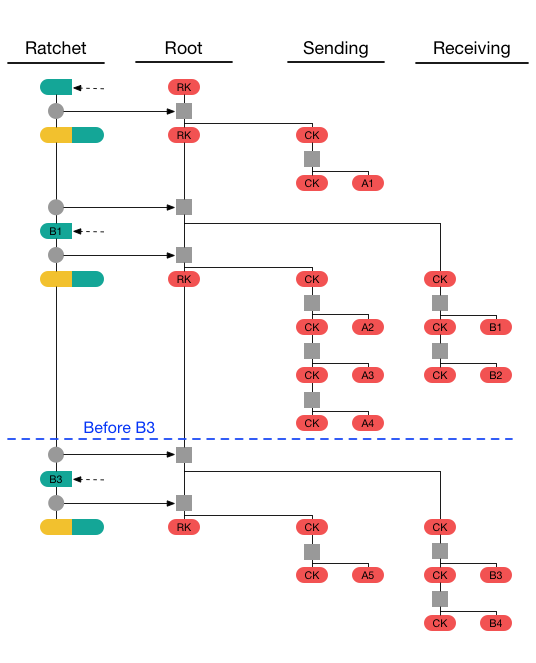
\includegraphics[width=12cm]{img/DR5.png}
\caption{}
\label{diagram:DR5} 
\centering
\end{center}
\end{figure}

\subsection{O que torna o protocolo do Signal superior?}
\textbf{FALAR DO QUE ESTA NA WIKEPEDIA NA PARTE DE ENCRYPTION PROTOCOLS }
\textbf{ADICIONAR UM BCD DAS PRIMITIVAS USADAS PARA ENCRIPTACAO}